% Versión para diapositiva (plantilla Semana ICG 2026): tamaño real 1:1, texto de 24 pt.
% Proceso 1 (proceso1mosaico.ipynb). Insertar en PowerPoint al 100 %.
\documentclass[border=2pt]{standalone}
\usepackage{iftex}
\ifPDFTeX
  \usepackage[utf8]{inputenc}
  \usepackage[T1]{fontenc}
  \usepackage[sfdefault]{carlito}
\else
  \usepackage{fontspec}
  \setmainfont{Carlito}[Extension=.ttf, UprightFont=*-Regular, BoldFont=*-Bold,
    ItalicFont=*-Italic, BoldItalicFont=*-BoldItalic]
\fi
\usepackage{tikz}
\usetikzlibrary{arrows.meta, positioning}

\definecolor{tinta}{HTML}{1B2A3A}
\definecolor{azul}{HTML}{1D5F83}
\definecolor{verde}{HTML}{5E8C45}
\definecolor{grisazul}{HTML}{7F9BB8}

\begin{document}
\fontsize{24}{29}\selectfont
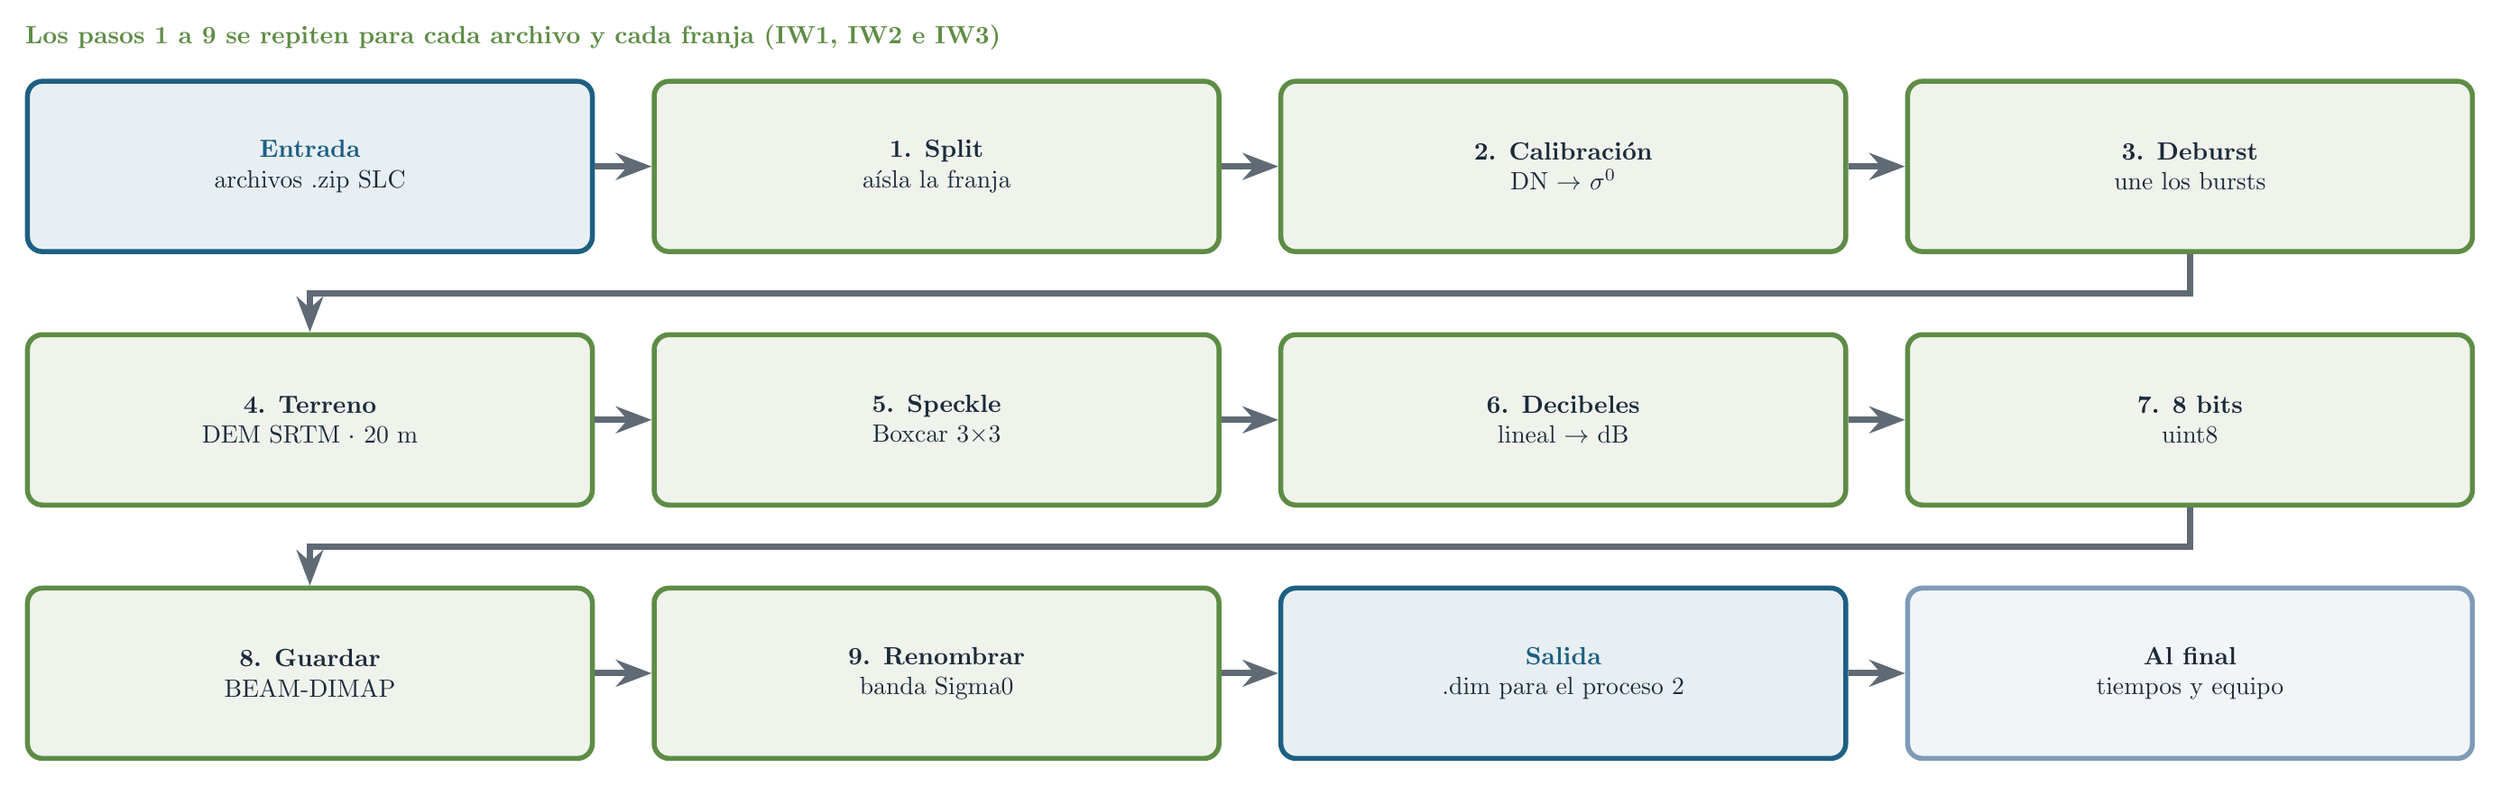
\begin{tikzpicture}[
  >=Stealth,
  caja/.style={rectangle, rounded corners=6pt, draw=#1, line width=2pt,
               fill=#1!10, text width=7.6cm, minimum height=2.4cm,
               align=flush center, text=tinta, inner sep=5pt},
  paso/.style={caja=verde},
  datos/.style={caja=azul},
  flecha/.style={->, line width=2.5pt, draw=tinta!70}
]
% fila 1
\node[datos] (in) {\textbf{\color{azul}Entrada}\\ archivos .zip SLC};
\node[paso, right=8mm of in] (p1) {\textbf{1. Split}\\ aísla la franja};
\node[paso, right=8mm of p1] (p2) {\textbf{2. Calibración}\\ DN $\rightarrow$ $\sigma^0$};
\node[paso, right=8mm of p2] (p3) {\textbf{3. Deburst}\\ une los bursts};
% fila 2
\node[paso, below=11mm of in] (p4) {\textbf{4. Terreno}\\ DEM SRTM · 20~m};
\node[paso, right=8mm of p4] (p5) {\textbf{5. Speckle}\\ Boxcar 3$\times$3};
\node[paso, right=8mm of p5] (p6) {\textbf{6. Decibeles}\\ lineal $\rightarrow$ dB};
\node[paso, right=8mm of p6] (p7) {\textbf{7. 8 bits}\\ uint8};
% fila 3
\node[paso, below=11mm of p4] (p8) {\textbf{8. Guardar}\\ BEAM-DIMAP};
\node[paso, right=8mm of p8] (p9) {\textbf{9. Renombrar}\\ banda Sigma0};
\node[datos, right=8mm of p9] (out) {\textbf{\color{azul}Salida}\\ .dim para el proceso 2};
\node[caja=grisazul, right=8mm of out] (res) {\textbf{Al final}\\ tiempos y equipo};

\foreach \a/\b in {in/p1, p1/p2, p2/p3, p4/p5, p5/p6, p6/p7, p8/p9, p9/out, out/res}
  \draw[flecha] (\a.east) -- (\b.west);
\draw[flecha] (p3.south) -- ++(0,-5.5mm) -| (p4.north);
\draw[flecha] (p7.south) -- ++(0,-5.5mm) -| (p8.north);

\node[anchor=south west, text=verde, font=\bfseries, inner sep=0pt]
  at ([yshift=4mm]in.north west)
  {Los pasos 1 a 9 se repiten para cada archivo y cada franja (IW1, IW2 e IW3)};
\end{tikzpicture}
\end{document}
